\begin{figure}[tbp]
    \centering
    \begin{subfigure}[b]{0.49\textwidth}
        \centering
        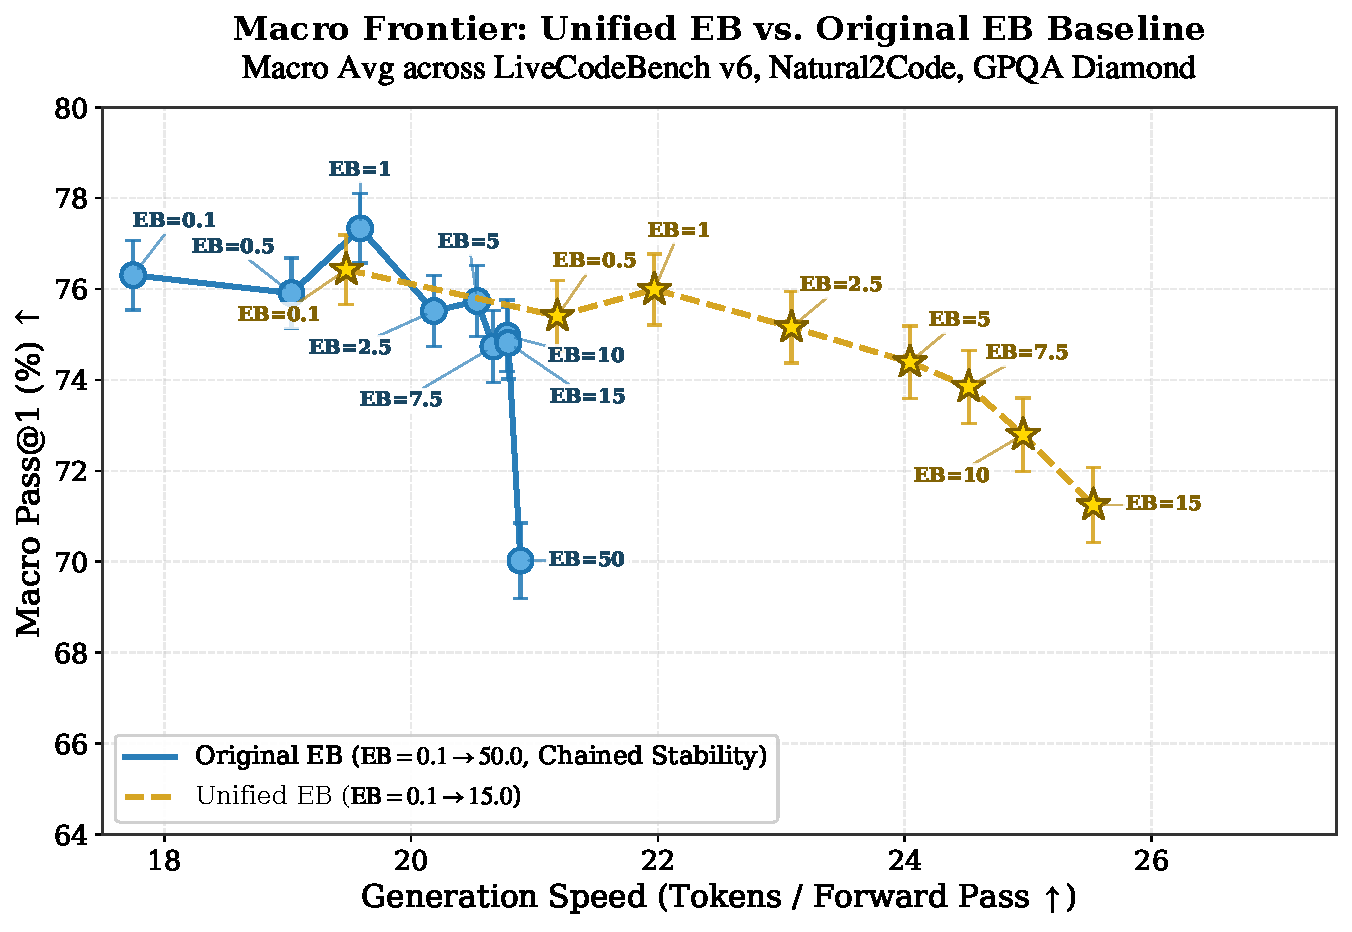
\includegraphics[width=\linewidth]{images/fig_macro_frontier_original_vs_unified.pdf}
        \caption{Original vs.\ unified stopping.}
        \label{fig:unified-vs-orig}
    \end{subfigure}
    \hfill
    \begin{subfigure}[b]{0.49\textwidth}
        \centering
        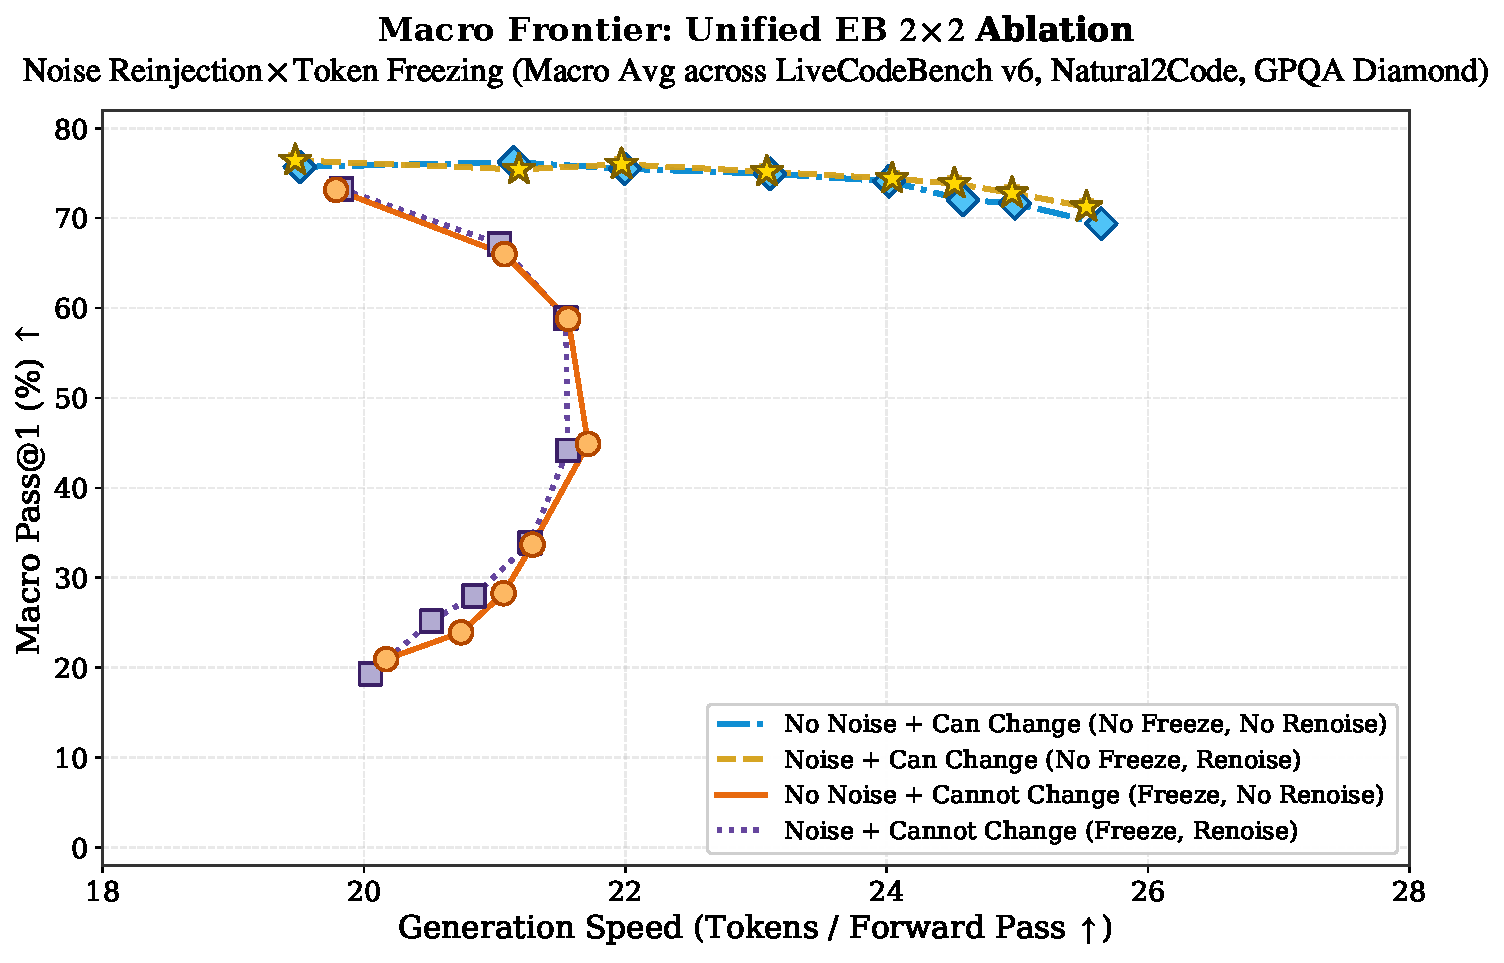
\includegraphics[width=\linewidth]{images/fig_macro_frontier_unified_ablation_2x2.pdf}
        \caption{Frozen vs.\ base EB sampler.}
        \label{fig:frozen-eb-frontier}
    \end{subfigure}

    \vspace{6pt}

    \begin{subfigure}[b]{\textwidth}
        \centering
        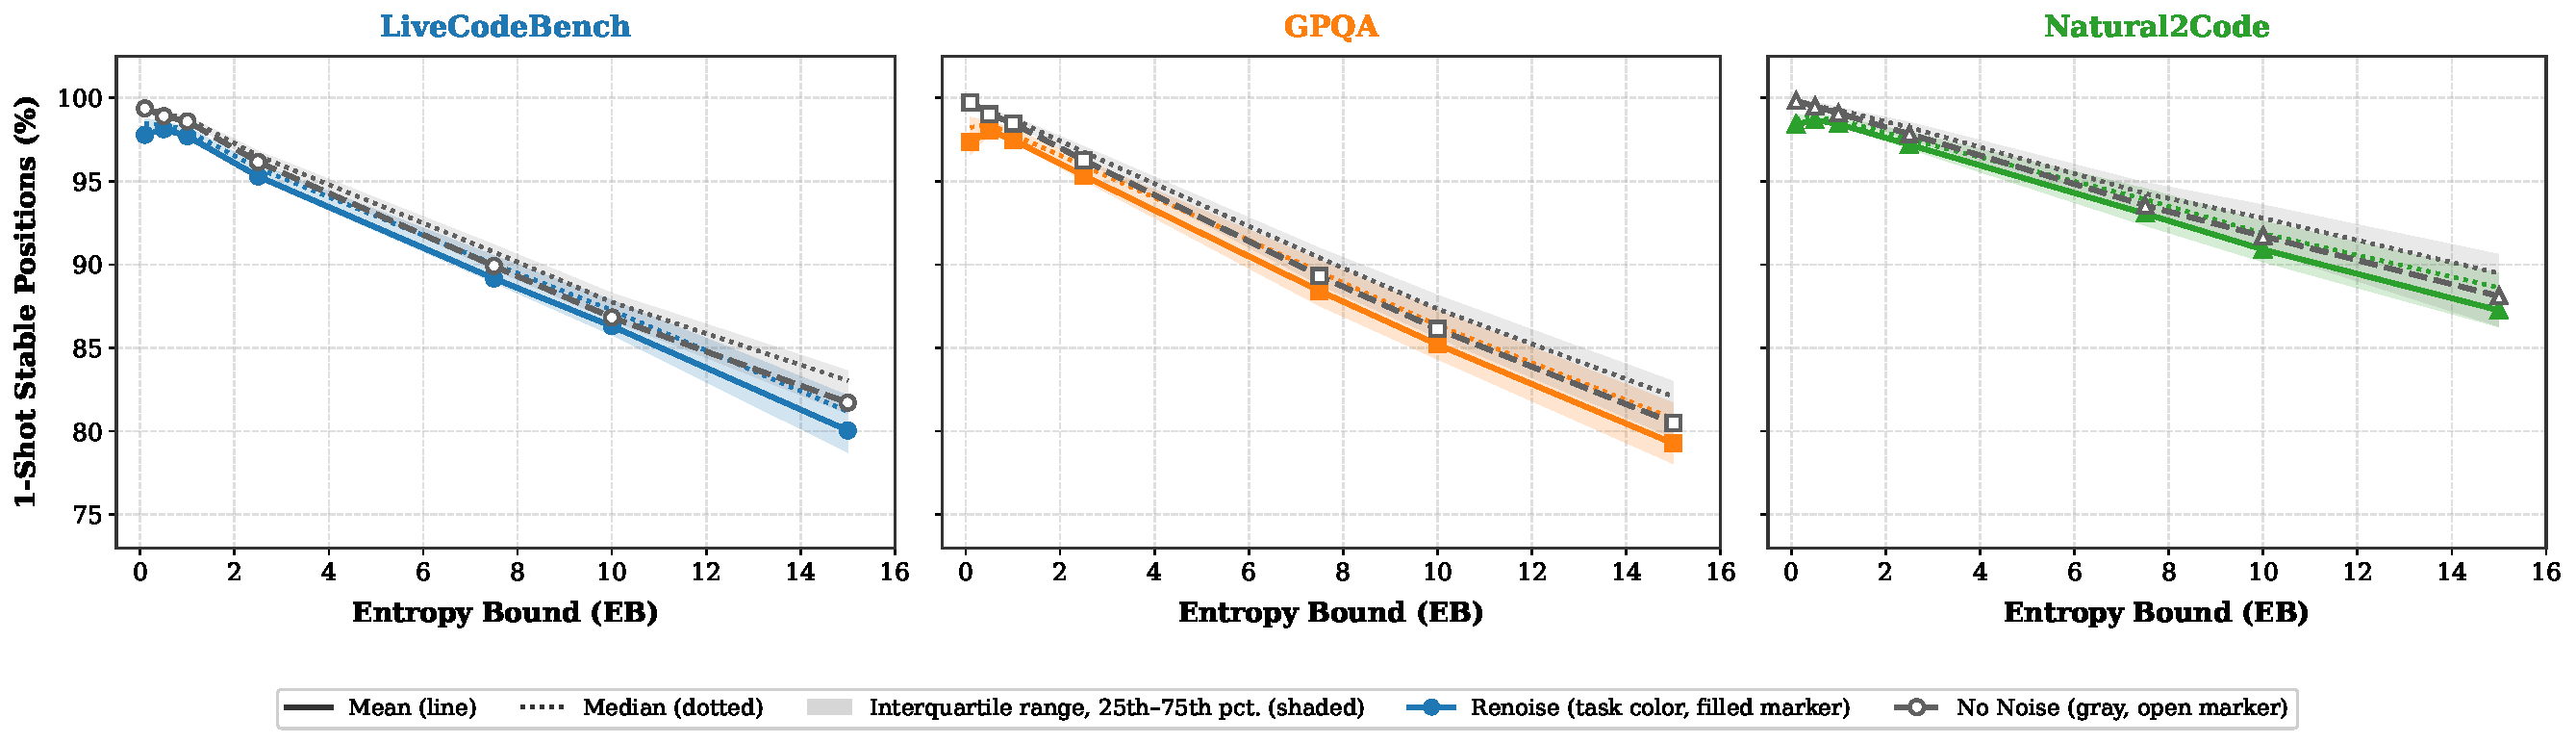
\includegraphics[width=\linewidth]{images/fig_1shot_stability_1x2_row.pdf}
        \caption{Stability of accepted tokens.}
        \label{fig:self-correct}
    \end{subfigure}
    \caption{\textbf{(a)} The unified stopping criterion matches the original at a slight speedup. \textbf{(b)} Pareto frontier of the modified EB sampler: larger entropy bounds trade performance for throughput, and the frozen variant degrades much faster than the base version, showing that the flexibility of the uniform diffusion process drives the frontier. \textbf{(c)} Accepted tokens are revised more often at higher entropy bounds (in both argmax and sampled-token stability), independent of renoising.}
    \label{fig:eb-frontiers}
\end{figure}